\chapter{Estado del Arte}
\thispagestyle{empty}

En el campo del aprendizaje automático, el tema de la estimación de la distancia en fotografías faciales ha ganado recientemente mucha atención. Se puede observar en la Figura \ref{fig16} la cantidad de publicaciones existentes en la base de datos Scopus \footnote{Las búsquedas se pueden consultar en el apéndice} que hacen referencia a la estimación de la SCD. Hay 441 publicaciones registradas desde 1992.

El número de publicaciones relacionadas con este tema, va aumentando a lo largo del tiempo, llegando a obtener un mayor número de publicaciones en 2020. Pese al aumento de publicaciones en este ámbito, es a partir del 2015 cuando se empiezan a aplicar las técnicas de aprendizaje profundo. Este aumento está relacionado con los avances tecnológicos que permiten aplicar nuevas técnicas y conocimientos. 

\begin{figure}[h]
	\centering
	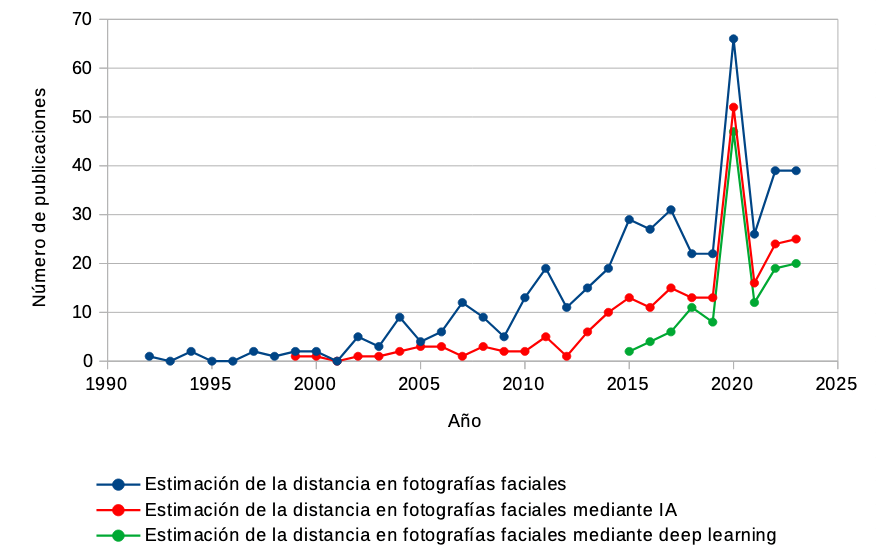
\includegraphics[scale=0.8]{imagenes/cap3/grafica_scopus5.png}
	\caption[Número de publicaciones sobre la estimación de la SCD.]{Número de publicaciones, en Scopus, relacionadas con la estimación de la distancia en fotografías faciales en función del año de publicación.}
	\label{fig16}
\end{figure}

\section{Primeros enfoques}

El primer método utilizado para abordar la estimación métrica de la SCD fue propuesto por Flores et al. \cite{28}, quienes proponen utilizar un conjunto de puntos de referencia faciales para calcular la distancia y la posición respecto a la cámara, en un rango que va desde los 10 cm hasta los 3 m.
Este método consiste en tomar una imagen 2D de una cara desconocida, identificar sus puntos de referencia faciales y compararlos con los puntos obtenidos de modelos faciales 3D conocidos. Luego, empleando el algoritmo EPnP \cite{29}, se determina la distancia entre la cámara y el sujeto. Esta técnica asume que los puntos de referencia no varían significativamente entre individuos, sino que tienden a agruparse en \textit{clusters}.

Sin embargo, este primer enfoque presenta algunas limitaciones, como la dependencia de conjuntos de datos en 3D (los cuales no siempre están disponibles), la mezcla de diferentes longitudes focales en un mismo conjunto de datos y la necesidad de reconocimiento manual de los puntos de referencia faciales.

Posteriormente, Burgos-Artizzu et al. \cite{30} introducen un método innovador que elimina la necesidad de anotación manual de los puntos de referencia de la imagen. En su lugar, estos puntos se estiman automáticamente mediante un enfoque de regresión conocido como \textit{Robust Cascaded Pose Regression} (RCPR) \cite{53}. Una vez que se han identificado los puntos de referencia faciales, se emplea un modelo automático de regresión para predecir la distancia entre la cámara y el sujeto en función de la posición relativa de estos puntos. Este regresor fue entrenado utilizando el conjunto de datos Caltech Multi-Distance Portraits (CMDP) \cite{54}, que consta de 53 retratos individuales tomados desde 7 distancias diferentes, que van desde 60 cm hasta 480 cm. Todos estos retratos están anotados manualmente con 55 marcas faciales.

Este método, sigue teniendo algunas limitaciones como el recorte de las imágenes (pérdida de resolución) o la única vista frontal.

Además de los métodos previamente citados, se han desarrollado otras técnicas para estimar la SCD basadas en características anatómicas como el tamaño facial \cite{32}, la separación entre los ojos \cite{33}, o una combinación de ambos factores \cite{34}.

\section{MediaPipe Iris}

MediaPipe Iris \footnote{https://blog.research.google/2020/08/mediapipe-iris-real-time-iris-tracking.html} es un modelo de aprendizaje automático desarrollado por investigadores de Google. Este modelo tiene la capacidad de rastrear puntos de referencia como el iris, la pupila y los contornos del ojo en tiempo real, utilizando únicamente una cámara RGB estándar y sin necesidad de utilizar ningún hardware especializado. Mediante el seguimiento de los puntos de referencia del iris, este modelo puede determinar la distancia métrica entre el sujeto y la cámara.

El modelo se basa en el diámetro horizontal del iris del ojo humano, el cual se mantiene relativamente constante en un rango de 11.7±0.5 mm en una amplia población. Esta característica, combinada con argumentos geométricos simples, permite al modelo estimar la distancia SCD.

Sin embargo, es importante destacar que este modelo presenta ciertas condiciones y limitaciones. Es útil únicamente en situaciones donde existan datos EXIF disponibles, se capturen imágenes frontales donde el iris sea visible, y los individuos se encuentren a una distancia de menos de 2 metros de la posición de la cámara.

\section{PerspectiveX}

PerspectiveX, desarrollado por Stephan et al. \cite{55}, es un método para la estimación de la SCD en imágenes faciales, diseñado para mejorar el proceso de superposición craneofacial.

Este método se basa en la localización de una característica anatómica específica, la longitud de la fisura palpebral, definida por dos puntos de referencia fácilmente identificables. 

Esta elección se justifica por varios aspectos: su clara visibilidad frontal, incluso cuando la cabeza experimenta un ligero giro hacia el lado más cercano a la cámara; su definición precisa, que garantiza una correcta medición; su mínima variabilidad, atribuible a restricciones evolutivas; su notable tamaño facial relativo, lo cual minimiza la probabilidad de errores en comparación con características más pequeñas, como el diámetro del iris; y su distribución normal, que contribuye a reducir el margen de error en las predicciones.

Además de la fisura palpebral, PerspectiveX requiere conocer el tipo de cámara, necesario para obtener las especificaciones de píxeles, así como la longitud focal de las lentes. Ambos datos pueden extraerse de las imágenes electrónicas mediante lectores EXIF disponibles en línea.

Finalmente, la estimación del SCD se realiza mediante la siguiente fórmula:

\begin{equation}
	SCD = f (1+\frac{A}{x \cdot y})
\end{equation}

donde: $f$, es la longitud focal de las lentes (mm); $A$, es la longitud real de la fisura palpebral (mm); $x$, es la longitud de la fisura palpebral en la foto (píxeles); $y$, son las especificaciones del tamaño del píxel del receptor de imagen (mm)

Dado que la longitud real de la fisura palpebral puede no estar disponible, se recurre al promedio de un grupo demográfico homogéneo en términos de sexo y edad, ya que se sabe que esta medida varía mínimamente debido a restricciones evolutivas.

Aunque PerspectiveX ofrece una estimación precisa de la SCD para una longitud focal conocida, presenta ciertas limitaciones, como la necesidad de intervención manual para marcar los puntos de referencia faciales y la falta de consideración de las rotaciones de cabeza superiores a 30°.

\section{FacialSCDnet}

FacialSCDnet, presentado por Bermejo et al. \cite{14}, es un método que estima la SCD directamente a partir de fotografías mediante el empleo de técnicas de aprendizaje profundo. La utilización de una arquitectura de redes neuronales profundas elimina una restricción crucial: la necesidad de detectar una característica anatómica específica para guiar el proceso de estimación. Esta capacidad permite que el método sea eficaz en la estimación de la SCD en cualquier posición de la cabeza, desde la frontal hasta el perfil lateral.

Para entrenar el modelo, se empleó un conjunto de datos compuesto por dos colecciones: 

\begin{itemize}
	\item Conjunto sintético: se generaron imágenes sintéticas 2D a partir de los modelos 3D de la base de datos Stirling ESRC 3D Face \footnote{Stirling ESRC 3D Face: https://pics.stir.ac.uk/ESRC/index.htm}. En particular, se utilizaron 315 modelos faciales de 54 individuos diferentes para generar aproximadamente 150.000 fotografías sintéticas.
	\item Conjunto de fotografías digitales: se adquirieron fotografías de 28 individuos siguiendo un protocolo de adquisición específico. Se consideraron 4 longitudes focales diferentes (27 mm, 35 mm, 55 mm, 85 mm) en formato full frame y se capturaron 12 distancias diferentes de la cámara al sujeto, que oscilaron desde 50 cm hasta 6 m. Además, se fotografiaron 7 posiciones distintas de la cabeza, desde el perfil izquierdo hasta el perfil derecho, con intervalos de rotación de 30º.
\end{itemize}

La función de pérdida empleada en el modelo se basa en el error absoluto medio de la distorsión facial relativa, calculada mediante la fórmula:

\begin{equation}
	Distorsion = \frac{\sum_{i=1}^{n} |y_i - x_i|}{n}
\end{equation}

donde $y_i$ son los valores reales (etiquetas) de la distorsión facial, y $x_i$ son los valores predichos de la distorsión facial, calculados a partir del factor de distorsión ($D_f$):

\begin{equation}
	D_f = \frac{1}{1 + \frac{SCD}{d}}
	\label{eq:df}
\end{equation}

En la ecuación \ref{eq:df}, $d = 12.6572 $ cm corresponde a un valor derivado de cálculos geométricos \cite{55} para obtener experimentalmente el factor de distorsión de una cabeza humana de tamaño promedio, según la SCD de la fotografía.

FacialSCDnet consta de 4 modelos de aprendizaje profundo, cada uno asociado a una longitud focal utilizada en el conjunto de datos. La estructura de cada CNN se basa en la arquitectura VGG-16, cuyos pesos se inicializan con los pre-entrenados en ImageNet \footnote{ImageNet: https://www.image-net.org/}. Para adaptar la arquitectura al problema de estimación de la SCD, se conservan los 5 bloques convolucionales, se elimina la cabeza superior de la red y se añaden 2 capas totalmente conectadas que se entrenan desde cero. Finalmente, la última capa del modelo consiste en una activación lineal que realiza la tarea de regresión.

El proceso de entrenamiento de los modelos constó de dos fases. En primer lugar, los modelos se entrenaron con el conjunto de datos sintético para aprender las relaciones entre la SCD y las características faciales. Posteriormente, se realizó un ajuste fino utilizando el conjunto de datos reales.

Los resultados obtenidos indican que las cuatro redes de FacialSCDnet son capaces de predecir con precisión la SCD, con errores promedio por debajo de 5 cm (MAE) o 3\% (MRE). Esta precisión en la predicción de la distancia métrica se traduce en un error promedio del 0.2\% al considerar la métrica de distorsión facial relativa. Estos resultados muestran que FacialSCDnet logra una estimación precisa de la SCD en fotografías faciales, superando a otros métodos existentes y demostrando su robustez y eficacia en diversas situaciones y condiciones.